\documentclass[conference]{IEEEtran}
\usepackage[style=ieee, backend=biber]{biblatex}

\ifCLASSINFOpdf
	\usepackage[pdftex]{graphicx}
	\graphicspath{{img/}}
	\DeclareGraphicsExtensions{.pdf,.jpg,.png}
\else
	\usepackage[dvips]{graphicx}
 	\graphicspath{{img/}}
	\DeclareGraphicsExtensions{.pdf,.jpg,.png}
\fi


% *** MATH PACKAGES ***
%
%\usepackage{amsmath}
% A popular package from the American Mathematical Society that provides
% many useful and powerful commands for dealing with mathematics.
%
% Note that the amsmath package sets \interdisplaylinepenalty to 10000
% thus preventing page breaks from occurring within multiline equations. Use:
%\interdisplaylinepenalty=2500
% after loading amsmath to restore such page breaks as IEEEtran.cls normally
% does. amsmath.sty is already installed on most LaTeX systems. The latest
% version and documentation can be obtained at:
% http://www.ctan.org/pkg/amsmath





% *** SPECIALIZED LIST PACKAGES ***
%
%\usepackage{algorithmic}
% algorithmic.sty was written by Peter Williams and Rogerio Brito.
% This package provides an algorithmic environment fo describing algorithms.
% You can use the algorithmic environment in-text or within a figure
% environment to provide for a floating algorithm. Do NOT use the algorithm
% floating environment provided by algorithm.sty (by the same authors) or
% algorithm2e.sty (by Christophe Fiorio) as the IEEE does not use dedicated
% algorithm float types and packages that provide these will not provide
% correct IEEE style captions. The latest version and documentation of
% algorithmic.sty can be obtained at:
% http://www.ctan.org/pkg/algorithms
% Also of interest may be the (relatively newer and more customizable)
% algorithmicx.sty package by Szasz Janos:
% http://www.ctan.org/pkg/algorithmicx




% *** ALIGNMENT PACKAGES ***
%
%\usepackage{array}
% Frank Mittelbach's and David Carlisle's array.sty patches and improves
% the standard LaTeX2e array and tabular environments to provide better
% appearance and additional user controls. As the default LaTeX2e table
% generation code is lacking to the point of almost being broken with
% respect to the quality of the end results, all users are strongly
% advised to use an enhanced (at the very least that provided by array.sty)
% set of table tools. array.sty is already installed on most systems. The
% latest version and documentation can be obtained at:
% http://www.ctan.org/pkg/array


% IEEEtran contains the IEEEeqnarray family of commands that can be used to
% generate multiline equations as well as matrices, tables, etc., of high
% quality.




% *** SUBFIGURE PACKAGES ***
%\ifCLASSOPTIONcompsoc
%  \usepackage[caption=false,font=normalsize,labelfont=sf,textfont=sf]{subfig}
%\else
%  \usepackage[caption=false,font=footnotesize]{subfig}
%\fi
% subfig.sty, written by Steven Douglas Cochran, is the modern replacement
% for subfigure.sty, the latter of which is no longer maintained and is
% incompatible with some LaTeX packages including fixltx2e. However,
% subfig.sty requires and automatically loads Axel Sommerfeldt's caption.sty
% which will override IEEEtran.cls' handling of captions and this will result
% in non-IEEE style figure/table captions. To prevent this problem, be sure
% and invoke subfig.sty's "caption=false" package option (available since
% subfig.sty version 1.3, 2005/06/28) as this is will preserve IEEEtran.cls
% handling of captions.
% Note that the Computer Society format requires a larger sans serif font
% than the serif footnote size font used in traditional IEEE formatting
% and thus the need to invoke different subfig.sty package options depending
% on whether compsoc mode has been enabled.
%
% The latest version and documentation of subfig.sty can be obtained at:
% http://www.ctan.org/pkg/subfig




% *** FLOAT PACKAGES ***
%
%\usepackage{fixltx2e}
% fixltx2e, the successor to the earlier fix2col.sty, was written by
% Frank Mittelbach and David Carlisle. This package corrects a few problems
% in the LaTeX2e kernel, the most notable of which is that in current
% LaTeX2e releases, the ordering of single and double column floats is not
% guaranteed to be preserved. Thus, an unpatched LaTeX2e can allow a
% single column figure to be placed prior to an earlier double column
% figure.
% Be aware that LaTeX2e kernels dated 2015 and later have fixltx2e.sty's
% corrections already built into the system in which case a warning will
% be issued if an attempt is made to load fixltx2e.sty as it is no longer
% needed.
% The latest version and documentation can be found at:
% http://www.ctan.org/pkg/fixltx2e


%\usepackage{stfloats}
% stfloats.sty was written by Sigitas Tolusis. This package gives LaTeX2e
% the ability to do double column floats at the bottom of the page as well
% as the top. (e.g., "\begin{figure*}[!b]" is not normally possible in
% LaTeX2e). It also provides a command:
%\fnbelowfloat
% to enable the placement of footnotes below bottom floats (the standard
% LaTeX2e kernel puts them above bottom floats). This is an invasive package
% which rewrites many portions of the LaTeX2e float routines. It may not work
% with other packages that modify the LaTeX2e float routines. The latest
% version and documentation can be obtained at:
% http://www.ctan.org/pkg/stfloats
% Do not use the stfloats baselinefloat ability as the IEEE does not allow
% \baselineskip to stretch. Authors submitting work to the IEEE should note
% that the IEEE rarely uses double column equations and that authors should try
% to avoid such use. Do not be tempted to use the cuted.sty or midfloat.sty
% packages (also by Sigitas Tolusis) as the IEEE does not format its papers in
% such ways.
% Do not attempt to use stfloats with fixltx2e as they are incompatible.
% Instead, use Morten Hogholm'a dblfloatfix which combines the features
% of both fixltx2e and stfloats:
%
% \usepackage{dblfloatfix}
% The latest version can be found at:
% http://www.ctan.org/pkg/dblfloatfix




% *** PDF, URL AND HYPERLINK PACKAGES ***
%
%\usepackage{url}
% url.sty was written by Donald Arseneau. It provides better support for
% handling and breaking URLs. url.sty is already installed on most LaTeX
% systems. The latest version and documentation can be obtained at:
% http://www.ctan.org/pkg/url
% Basically, \url{my_url_here}.




% *** Do not adjust lengths that control margins, column widths, etc. ***
% *** Do not use packages that alter fonts (such as pslatex).         ***
% There should be no need to do such things with IEEEtran.cls V1.6 and later.
% (Unless specifically asked to do so by the journal or conference you plan
% to submit to, of course. )


% correct bad hyphenation here
\hyphenation{op-tical net-works semi-conduc-tor}


\bibliography{paper.bib}


\begin{document}
\title{Mimicry in Online Conversations: An Exploratory Study of Linguistic Analysis Techniques}


% author names and affiliations
% use a multiple column layout for up to three different
% affiliations
\author{\IEEEauthorblockN{Tom Carrick, Awais Rashid, Paul J Taylor}
\IEEEauthorblockA{Security Lancaster / CREST\\
Lancaster University\\
Lancaster, United Kingdom\\
Email: \{t.carrick, a.rashid, p.j.taylor\} @lancaster.ac.uk}
\and
\IEEEauthorblockN{Adam Joinson}
\IEEEauthorblockA{???\\
University of Bath\\
Bath, United Kingdom\\
Email: a.joinson@bath.ac.uk}}

% conference papers do not typically use \thanks and this command
% is locked out in conference mode. If really needed, such as for
% the acknowledgment of grants, issue a \IEEEoverridecommandlockouts
% after \documentclass

% for over three affiliations, or if they all won't fit within the width
% of the page, use this alternative format:
% 
%\author{\IEEEauthorblockN{Michael Shell\IEEEauthorrefmark{1},
%Homer Simpson\IEEEauthorrefmark{2},
%James Kirk\IEEEauthorrefmark{3}, 
%Montgomery Scott\IEEEauthorrefmark{3} and
%Eldon Tyrell\IEEEauthorrefmark{4}}
%\IEEEauthorblockA{\IEEEauthorrefmark{1}School of Electrical and Computer Engineering\\
%Georgia Institute of Technology,
%Atlanta, Georgia 30332--0250\\ Email: see http://www.michaelshell.org/contact.html}
%\IEEEauthorblockA{\IEEEauthorrefmark{2}Twentieth Century Fox, Springfield, USA\\
%Email: homer@thesimpsons.com}
%\IEEEauthorblockA{\IEEEauthorrefmark{3}Starfleet Academy, San Francisco, California 96678-2391\\
%Telephone: (800) 555--1212, Fax: (888) 555--1212}
%\IEEEauthorblockA{\IEEEauthorrefmark{4}Tyrell Inc., 123 Replicant Street, Los Angeles, California 90210--4321}}




% use for special paper notices
%\IEEEspecialpapernotice{(Invited Paper)}




% make the title area
\maketitle

% As a general rule, do not put math, special symbols or citations
% in the abstract
\begin{abstract}
The Interactive Alignment Model is the prevailing theory of
[I probably need some help phrasing this].
In this study we investigate how several linguistic alignment techniques can be used
to detect mimicry at the lexical, syntactic and situational levels of the
Interactive Alignment Model.

We show that [something].
\end{abstract}

% no keywords




% For peer review papers, you can put extra information on the cover
% page as needed:
% \ifCLASSOPTIONpeerreview
% \begin{center} \bfseries EDICS Category: 3-BBND \end{center}
% \fi
%
% For peerreview papers, this IEEEtran command inserts a page break and
% creates the second title. It will be ignored for other modes.
\IEEEpeerreviewmaketitle



\section{Introduction}
% no \IEEEPARstart

Mimicry in online conversations is an important area of research [something about insider threats
and maybe something about improving outcomes of tasks, using mimicry in AI, etc.]

There are a number of measures designed to capture mimicry in text, [something something], and some
efforts have been made to compare and trial these techniques. However, few of these techniques are 
grounded what cognitive science knows about how mimicry works within humans.

This perspective is important so that each measure is grounded in reality.
Moreover, it suggests [does it?] that the best approach may be to combine existing measures to create
a more holistic measure. [don't like any of this wording].

Of the measures discussed in this paper, only one has attempted to measure alignment with this in mind
and some, such as LSM seem to work outside of the theory altogether.

This paper aims to compare how well existing linguistic analysis techniques work to detect mimicry in 
relation to the Interactive Alignment Model. Further, we also look at some existing techniques that 
have not previously been used to detect mimicry and discuss their viability.

[Not sure what else to put here. Section II does this, section III looks at that type thing?]


\section{Related Work}
This paper draws from many sources for its measures. The most similar piece of work is a comparison
of several methods\cite{xu2015evaluation}, some discussed in this paper. It does not, however, try
to compare the accuracy of the measures, rather, it [does some stuff I don't understand that well,
seems like it looks at some statistical properties?]

[Not sure what else to mention here]


\section{The Interactive Alignment Model}
The Interactive Alignment Model (IAM)\cite{pickering2004toward} is an attempt to model alignment in
conversations. It consists of six layers, which with the exception of the top layer, the situation
model, are all representations of some aspect of speech.

\begin{enumerate}
	\item The situation model --- a representation of the situation being discussed
	\item The semantic representation --- the meaning of the utterance
	\item The syntactic representation --- the sentence structure
	\item The lexical representation --- the choice of words used
	\item The phonological representation --- [I have no idea how to describe the difference between
		phonology and phonetics]
	\item The phonetic representation --- something
\end{enumerate}

The phonological and phonetic layers are ignored by this paper as they do not relate to written text.

The theory states that alignment "percolates" between layers such that increased alignment in one layer
will lead to increased alignment in other layers.

\begin{figure*}
	\caption{The interactive alignment model}
	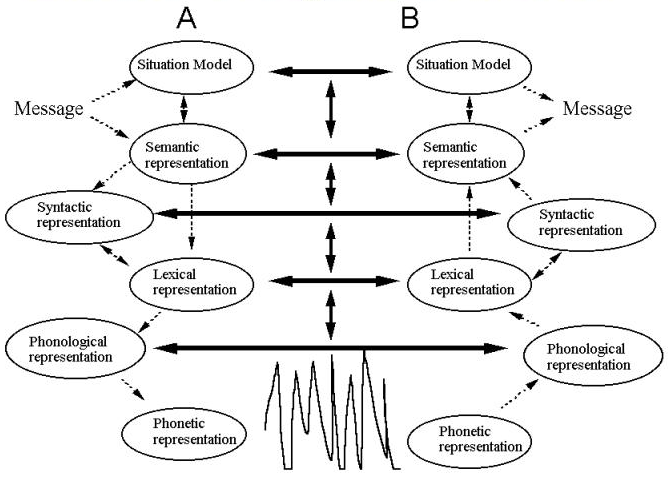
\includegraphics[width=\textwidth]{iam}
\end{figure*}


\section{Method}

\subsection{Data}
The dataset consists of 103 dyadic conversations taken from Twitter. Tweets were found via Twitter's 
search API, using English language and being a reply as criteria. We then work up the chain of tweets 
until we hit the end, or a third interlocutor is found, at which point the conversation is cut off and 
kept, as long as there are no fewer than 10 tweets in the conversation. 200 tweets were found using 
this method. Of these, 62 were removed as they were not true conversations (either monologues or 
collaborative fiction writing/roleplay). 18 conversations were removed as they had significant amounts 
of non-English text, and 17 conversations involved bots and were also removed.

The data is processed as follows:
\begin{itemize}
	\item Screen names at the start of the message are removed. These are just the names of the 
		  interlocutors and only add noise.
	\item All URLs are replace with the string '[URL]'.
	\item HTML entities such as \&amp; are converted to plain text (\&).
	\item Any adjacent messages by the same author are merged together such that each message always
	      alternates between the two interlocutors.
\end{itemize}

The data was classified by three PhD students at Lancaster University with backgrounds in mimicry. Each 
conversation was classified for lexical, syntactic and semantic mimicry on a three point scale where 0 
represents no mimicry, 1 represents low levels of mimicry at that layer, and 2 represents high levels 
of mimicry.

Each measure, with exceptions noted in following subsections [Probably just HAM at this point],
is then run against the data such that each message from author A is compared with each message from 
author B that occurred before the original message.
\footnote{[I could probably make my github repo public and put a link to the code here?]}

[Need to justify dataset and discuss limitations]


\subsection{Lexical}
Lexical stuff.

\subsubsection{LILLA}
Lexical Indiscriminate Local Linguistic Alignment (LILLA)\cite{wang2014linguistic, xu2015evaluation}
is a measure that explicitly works at the lexical layer. It gives the probability that a word from the 
prime document will appear at a particular position in the target document. It is defined as:

\[LILLA(target, prime) = \frac{p(target|prime)}{p(target)}\]


\subsubsection{HAM}
The Hierarchical Alignment Model (HAM)\cite{doyle2016robust} ...


\subsection{Syntactic}
Syntactic stuff.

\subsubsection{SILLA}
Syntactic Indiscriminate Local Linguistic Alignment (SILLA)

\subsubsection{SHAM}
SHAM


\subsection{Semantic}
Semantic

\subsubsection{word2vec}
word2vec\cite{mikolov2013distributed}

\subsubsection{doc2vec}
doc2vec\cite{le2014distributed}.


\subsection{Other Measures}
Other

\subsubsection{Linguistic Style Matching}
LSM\cite{niederhoffer2002linguistic}

\subsubsection{Zelig}
Zelig\cite{jones2014finding}


\section{Results}
Still not sure how to compare everything.

% An example of a floating figure using the graphicx package.
% Note that \label must occur AFTER (or within) \caption.
% For figures, \caption should occur after the \includegraphics.
% Note that IEEEtran v1.7 and later has special internal code that
% is designed to preserve the operation of \label within \caption
% even when the captionsoff option is in effect. However, because
% of issues like this, it may be the safest practice to put all your
% \label just after \caption rather than within \caption{}.
%
% Reminder: the "draftcls" or "draftclsnofoot", not "draft", class
% option should be used if it is desired that the figures are to be
% displayed while in draft mode.
%
%\begin{figure}[!t]
%\centering
%\includegraphics[width=2.5in]{myfigure}
% where an .eps filename suffix will be assumed under latex, 
% and a .pdf suffix will be assumed for pdflatex; or what has been declared
% via \DeclareGraphicsExtensions.
%\caption{Simulation results for the network.}
%\label{fig_sim}
%\end{figure}

% Note that the IEEE typically puts floats only at the top, even when this
% results in a large percentage of a column being occupied by floats.


% An example of a double column floating figure using two subfigures.
% (The subfig.sty package must be loaded for this to work.)
% The subfigure \label commands are set within each subfloat command,
% and the \label for the overall figure must come after \caption.
% \hfil is used as a separator to get equal spacing.
% Watch out that the combined width of all the subfigures on a 
% line do not exceed the text width or a line break will occur.
%
%\begin{figure*}[!t]
%\centering
%\subfloat[Case I]{\includegraphics[width=2.5in]{box}%
%\label{fig_first_case}}
%\hfil
%\subfloat[Case II]{\includegraphics[width=2.5in]{box}%
%\label{fig_second_case}}
%\caption{Simulation results for the network.}
%\label{fig_sim}
%\end{figure*}
%
% Note that often IEEE papers with subfigures do not employ subfigure
% captions (using the optional argument to \subfloat[]), but instead will
% reference/describe all of them (a), (b), etc., within the main caption.
% Be aware that for subfig.sty to generate the (a), (b), etc., subfigure
% labels, the optional argument to \subfloat must be present. If a
% subcaption is not desired, just leave its contents blank,
% e.g., \subfloat[].


% An example of a floating table. Note that, for IEEE style tables, the
% \caption command should come BEFORE the table and, given that table
% captions serve much like titles, are usually capitalized except for words
% such as a, an, and, as, at, but, by, for, in, nor, of, on, or, the, to
% and up, which are usually not capitalized unless they are the first or
% last word of the caption. Table text will default to \footnotesize as
% the IEEE normally uses this smaller font for tables.
% The \label must come after \caption as always.
%
%\begin{table}[!t]
%% increase table row spacing, adjust to taste
%\renewcommand{\arraystretch}{1.3}
% if using array.sty, it might be a good idea to tweak the value of
% \extrarowheight as needed to properly center the text within the cells
%\caption{An Example of a Table}
%\label{table_example}
%\centering
%% Some packages, such as MDW tools, offer better commands for making tables
%% than the plain LaTeX2e tabular which is used here.
%\begin{tabular}{|c||c|}
%\hline
%One & Two\\
%\hline
%Three & Four\\
%\hline
%\end{tabular}
%\end{table}


% Note that the IEEE does not put floats in the very first column
% - or typically anywhere on the first page for that matter. Also,
% in-text middle ("here") positioning is typically not used, but it
% is allowed and encouraged for Computer Society conferences (but
% not Computer Society journals). Most IEEE journals/conferences use
% top floats exclusively. 
% Note that, LaTeX2e, unlike IEEE journals/conferences, places
% footnotes above bottom floats. This can be corrected via the
% \fnbelowfloat command of the stfloats package.


\section{Conclusion and Future Work}
The conclusion goes here.

\section{Discussion}
Discussion


% use section* for acknowledgment
\section*{Acknowledgment}
The authors gratefully acknowledge a grant from CREST (probably need to find the name of this).


% trigger a \newpage just before the given reference
% number - used to balance the columns on the last page
% adjust value as needed - may need to be readjusted if
% the document is modified later
%\IEEEtriggeratref{8}
% The "triggered" command can be changed if desired:
%\IEEEtriggercmd{\enlargethispage{-5in}}

\printbibliography

\end{document}
